
Our first-order model can be used to describe the response of a temperature sensor to changes in the ambient environment.  This is analogous to our ``car'' model in that the temperature sensor has thermal inertia (analogous to the mass of our ``car'') and thermal resistance (analogous to the drag of our ``car'').  

\subsection{Mathematical Model}
Suppose we have a bulb thermometer that is at equilibrium the instant before it is plunged into boiling water.  The measured temperature will not instantly move to \unit[100]{$^{\circ}$C}, but instead the temperature of the device ($T(t)$) will move toward the new equilibrium over time.  The speed of that response is determined by the inertia and resistance of the system.

Figure~\ref{f:therm} illustrates how we might analyze this system.  Newton's law of cooling says that ``the rate of heat loss of a body is proportional to the difference in temperatures between the body and the surroundings'', or, stated mathematically,
\begin{equation}
\dot{Q}=hA (T_f(t)-T(t))
\end{equation}
where $\dot{Q}$ is the rate of heat transfer, $h$ is the heat transfer coefficient, $A$ is the surface area of the thermometer, $T_f(t)$ is temperature of the surroundings and $T(t)$ is the temperature of the thermometer.  Furthermore the thermal energy in the thermometer mass is $Q=C(T(t))$ where $C$ is the total heat capacity (the product of the mass ($m$) and the specific heat capacity of the material ($c_p$)).  Putting this together we can come up with a first-order model for a thermometer
\begin{equation}
\label{e:therm}
\dot{T}(t)= \frac{hA}{C}(T_f(t)-T(t)).
\end{equation}

\begin{figure}[hbt]
\centering
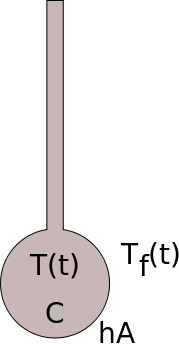
\includegraphics[width=0.20\textwidth]{thermometer.png}
\caption{Illustration of a simple model of the response of a thermometer.}
\label{f:therm}
\end{figure}

\begin{ex}
Using (\ref{e:therm}) rearrange the terms so that the expression has the same form as our canonical first-order model (\ref{e:first}).    What is the input to our model?  What is the output of our model?  What is the time constant of this model?  What is the steady-state temperature predicted by this model?
\end{ex}

\ifsolutions
\begin{soln}
\[ 
\dot{T}(t)+\frac{hA}{C}(T(t)) = \frac{hA}{C} (T_f(t)) 
\]
where $\tau = \frac{C}{hA}$.
\begin{itemize}
\item The input is the temperature of the surrouding fluid---$T_f(t)$.
\item The output is the temperature of the sensor---$T(t)$.
\item The time constant is $\tau = \frac{C}{hA}$
\item The steady state temperature is $T_{ss}=T_f$.
\end{itemize}
\end{soln}
\fi
